\chapter{Análise Bibliográfica sobre Simulação de Big Data na economia, por Tong Zhou\label{chap:bibliometria:Tong00020}}


\section{Planejamento do estudo}

O Big Data estuda, analisa e trata de um conjunto de dados maior e mais complexo que as processadas em sistemas tradicionais. Isso permite a resolução de problemas que não eram possíveis anteriormente.
Na economia, ele é utilizado desde as informações de consumo das pessoas, o preço dos produtos ao longo do tempo à medição do índice de inflação de um país.
Esta pesquisa busca encontrar quais áreas estão sendo mais estudadas nos últimos anos, em outras palavras, quais são mais relevantes para a economia, e quais países se destacam nestes estudos.

Algumas perguntas para basear a pesquisa são:
\begin{itemize}
    \item Quais são os temas mais abordados nos artigos?
    \item Quais são os autores mais relevantes e em quais regiões predomina a pesquisa nesta área?
\end{itemize}


\subsection{O que já existe de pesquisa bibliométrica sobre esse tema?}
 Foi encontrado um estudo bibliométrico de publicações sobre Big Data e economia em  \cite{nobre_scientific_2017}. Ele faz um estudo focado na aplicação de big data e internet das coisas na economia circular. Nesta pesquisa a busca será feita em um contexto mais geral. 


\subsection{Uso do Bibliometrix e Biblioshiny}

A pesquisa bibliométrica foi realizada com o uso do RStudio, foram usados o pacote \textit{Bibliometrix} e o aplicativo \textit{Biblioshiny} a partir do que foi apresentado em aula. Através do acesso café do portal Periódicos CAPES, foi utilizada a \textit{Web of Science} para extrair os artigos usados na pesquisa.


\subsection{Limitações} 

Nesta tarefa foram feitas duas buscas na base de dados WoS, pois a primeira, de 700 artigos, o número de artigos não foi suficiente para gerar gráficos apresentáveis. Sendo utilizada a segunda, de 1.265 artigos.


\section{Coleta de dados}

A coleta de dados feita usando o Web Of Science (WoS) no dia 03 de fevereiro de 2022, acessado por meio do Portal de Periódicos da CAPES. Foram feitas buscas nas coleções \textbf{Science  Citation  Index  Expanded (SCI -EXPANDED)}, \textbf{Social Sciences  Citation  Index (SSCI)}, \textbf{Conference Proceedings Citation Index-Science (CPI-S)} e \textbf{Emerging Sources Citation Index(ESCI)}. 

\subsection{Query de Busca}

Foi usada a query de busca abaixo: 


\lstinputlisting[numbers=left,basicstyle=\normalsize\ttfamily,caption={Query de busca sobre Processamento de Linguagem Natural.},label=query]{experiments/Tong00020/PesqBibliogr/SimulacaoMultiagente/WoS-20220203/query.txt}



\subsubsection{Explicação para os termos de busca usados}

Nesta busca, foi utilizado primeiro, duas palavras big data e economy (economia), que são os assuntos principais da pesquisa.%%%

Foram colocados também, o filtro para que apenas artigos de 2010 a 2022 entrem na pesquisa. No final, foram encontrados 1265 artigos.


\subsection{Registros recuperados}

Os 1.265 registros obtidos como resultado da busca encontram-se em \url{https://github.com/jhcf/Comput-Experim-20212/experiments/Tong00020/PesqBibliogr/SimulacaoMultiagente/WoS-20220203/1265records.txt}

Foram utilizadas as opções exporta em arquivo .txt e \textit{export full record / Gravar Conteúdo: Seleção personalizada}, com todos os 29 campos disponíveis. Os 1.265 registros foram recuperados em dois blocos de até 1.000 registros por vez (1-1000, 1001-1265).


\begin{figure}[ht]
    \centering
    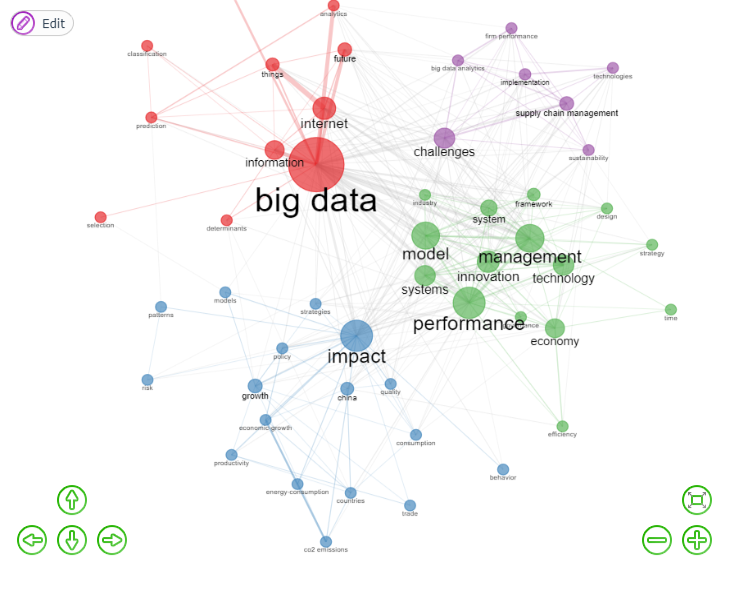
\includegraphics[width=11cm]{experiments/Tong00020/PesquisaBibliometrica/Conceptual Structure/MASSA@Tong00020-Co-occurrence Network}
    \caption{Rede de co-ocorrência de palavras chaves}
    \label{fig:rede}
\end{figure}



\section{Análise dos dados}

\subsection{Filtragem de registros}

Sobrou 1.168 artigos ao colocar apenas 'ARTICLE' como tipo de documento com o uso filtro do biblioshiny. Os tipos de documento 'ARTICLE; BOOK CHAPTER', 'ARTICLE; DATA PAPER', 'ARTICLE; EARLY ACCESS', 'ARTICLE; PROCEEDINGS PAPER' e 'ARTICLE; RETRACTED PUBLICATION' foram deletados.



\subsection{Análise descritiva do \textit{dataset}} 
%MASSA@Tong00020}

As informações mais gerais sobre o \textit{dataset} MASSA@Tong0020 são as seguintes:
\begin{description}
    \item[\textit{Timespan}] Os artigos da busca foram publicados a partir de 2010.
    \item [\textit{Sources (Journals, Books, etc)}] São 719 fontes publicaram os documentos no \dataset\. Em média, cada \textit{scientific journal} publicou $1.168/719=1.62$ artigos.%%%
     \item [\textit{Average years from publication}] A média do tempo de publicação dos artigos no dataset é de 3.25 anos.
     \item [\textit{Average citations per documents}] Cada artigo no dataset foi citado, em média 16.79 vezes.
     \item [\textit{Average citations per year per doc}] Após publicado, cada um dos 1.168 artigos do dataset foi citado 3.421 vezes por ano, em média.
    \item [\textit{References}] O dataset contém 61.413 referências citada.
    \item [\textit{Keywords Plus (ID)}] 2.857 distintas palavras-chave do tipo Keywords Plus (ID).
    \item [\textit{Author's Keywords (DE)}] 4.420 distintas palavras-chave indicadas pelos autores foram encontradas no \textit{dataset}.
     \item [\textit{Authors}] 10.181 nomes distintos de autores foram encontrados no \textit{dataset}.
    \item [\textit{Author Appearances}] Os 10.181 distintos (nomes de) autores foram encontrados 13.591 vezes, como autores de artigos.
    \item [\textit{Authors of single-authored documents}] Dentre os 10.181 distintos (nomes de) autores encontrados, 167 deles editaram artigos individualmente, isso é, sem co-autores.
    \item [\textit{Authors of multi-authored documents}] Dentre os 10.181 distintos (nomes de) autores encontrados, 10.014 deles editaram artigos com um ou mais co-autores"
    \item [\textit{Single-authored documents}] Dentre os 1.168 documentos presentes no \dataset\, 173 foram escritos por um único autor, e os 995 restantes foram elaborados em co-autoria.
    \item [\textit{Documents per Author}] Dentre os 10.181 distintos (nomes de) autores, cada um publicou em média 0,115 artigos.
    \item [\textit{Authors per Document}] Cada um dos 1.168 documentos presentes no \textit{dataset}  foi autorado com 8.72 autores em média ($10.181 / 1.168 = 8.72$).
    \item [\textit{Co-Authors per Documents}] As 13.591 aparições de (nomes de) autores (``Author Appearances''), sem distribuem, em média 11.6 vezes para os 1.168 documentos do \textit{dataset}.
    \item [\textit{Collaboration Index}] Os 10.181 (nomes de) autores que editaram artigos com um ou mais co-autores, colaboraram em media 10.1 vezes para editar os 1.168 artigos elaborados em co-autoria, gerando, assim, um índice de colaboração 10.1. 
    
\end{description}

     
\subsection{Evolução da Produção Científica}
A figura \ref{fig:ev-s-p} apresenta a evolução da produção científica entre 2010 e 2022, podemos ver que há uma forte tendência de crescimento a partir de 2016.

\begin{figure}[ht]
    \centering
    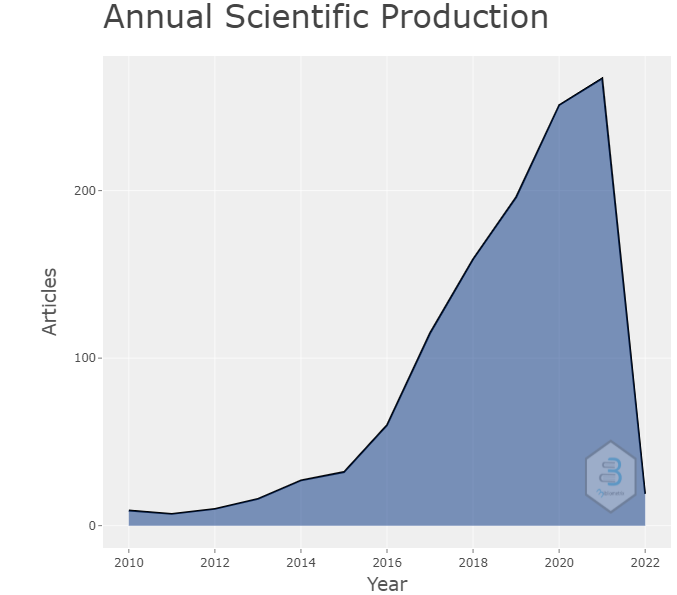
\includegraphics[width=12cm]{experiments/Tong00020/PesquisaBibliometrica/DataSet/MASSA@Tong00020-Annual Scientific Production.png}
    \caption{Evolução da produção científica presente no dataset}
    \label{fig:ev-s-p}
\end{figure}

     
\subsubsection{Interpretação do Crescimento}

O enorme aumento na taxa de crescimento do dataset, mostra a importância deste assunto nas pesquisas atuais. Principalmente, quando o uso de novas tecnologias está cada vez mais presente na economia mundial.

\subsection{Evolução das Citações}
A figura \ref{fig:average-cit} apresenta a evolução da média de citações dos artigos no dataset. Nota-se grandes quantidades de citações no ano de 2013 e, em uma proporção menor, no ano de 2017. Provavelmente pelo dataset apresentar um artigo com um grande de citações.

\begin{figure}[ht]
    \centering
    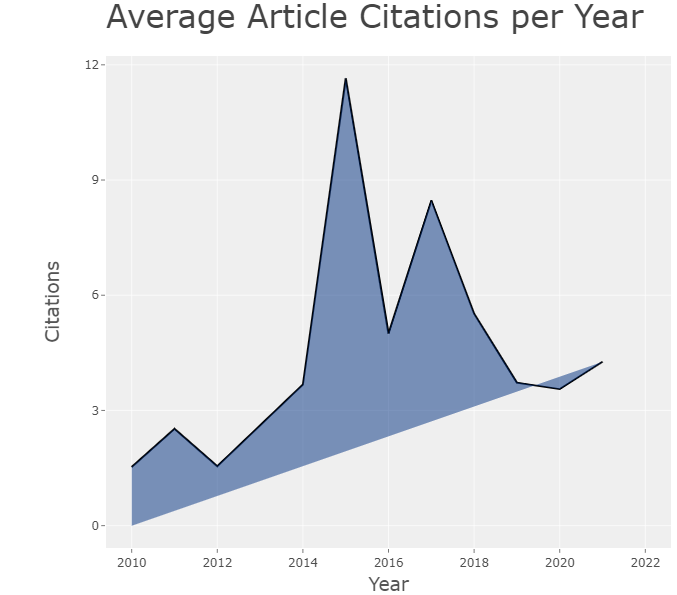
\includegraphics[width=12cm]{experiments/Tong00020/PesquisaBibliometrica/DataSet/MASSA@Tong00020-Average Citations per Year.png}
    \caption{Evolução das citações no dataset}
    \label{fig:average-cit}
\end{figure}

\subsubsection{Interpretação das Citações}
Além dos picos apresentados no gráfico, percebe-se que há um aumento na quantidade de citações de 2010 à 2022.

\subsection{\textit{Three-Field Plots (Sankey diagram)}}
A figura \ref{fig:g-tres} apresenta um gráfico que mostra a afinidade entre os três conjuntos de atributos,  referências, afiliações e palavras-chaves.

Na primeira coluna apresenta as 20 referências mais citadas; a segunda, as 20 afiliações(universidades, academias, instituições, etc) mais proeminentes e; a terceira, as 20 palavras-chaves mais usadas.

\begin{figure}[ht]
    \centering
    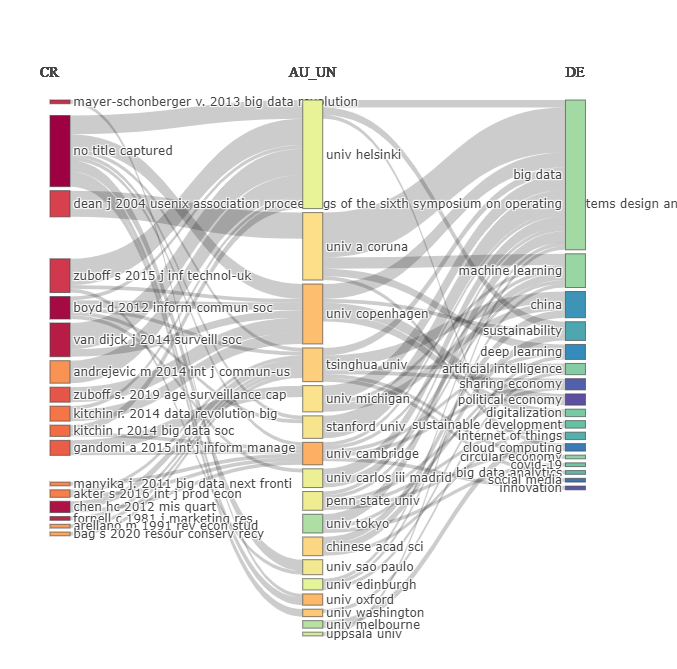
\includegraphics[width=12cm]{experiments/Tong00020/PesquisaBibliometrica/DataSet/MASSA@Tong00020-Three Fields Plot Affiliations References Keywords.png}
    \caption{Gráfico dos “Três Campos” (Sankey plot) de referências, afiliações e palavras-chaves}
    \label{fig:g-tres}
\end{figure}

\subsubsection{Interpretação da figura}
Na figura \ref{fig:g-tres} podemos ver que as publicações estão bem divididas entre os continentes. A mais proeminente, a Universidade de Helsinki, é da Finlândia(Ásia) e a segunda mais proeminente, a Universidade da Corunha (University of A Coruña), é da Espanha, Europa.

Observa-se na figura, que os artigos mais citados encontram-se publicados entre 2014 e 2015 e a maioria delas foi publicada pela Universidade de Helsinki. Provavelmente, foi uma época de muitas pesquisas nesta área na universidade.

Nas palavras-chaves, big data, machine learning e China são as mais usadas. Deve-se, principalmente, pelo uso e investimentos cada vez maiores nessa área no país asiático.


\subsection{Autores mais relevantes}
Apresentamos a seguir comentários sobre os autores mais citados nos trabalhos.


\subsection{Refinamento da coleta de dados}


\section{Resultados e interpretação}
Nesta pesquisa podemos concluir que pesquisas sobre o uso do Big Data na economia tem aumentado e muito nos últimos anos em todo o mundo. 